\section{Objektdetektoren}

Ein Teilziel der Machbarkeitsstudie ist es, anhand vorbestimmter Kriterien eine ausgewählte Menge von Objektdetektoren zu vergleichen. Um im Laufe der Arbeit zu verstehen, wie diese Auswahl zu Stande kommt und wie sich bestimmte Ergebnisse im Vergleich begründen lassen, ist eine Einführung in die unterschiedlichen Architekturen der Objektdetektoren unumgänglich. 

\subsection*{Regional Convolutional Neural Networks}

\textit{Regional Convolutional Neural Networks} (R-CNNs) vertreten den Ansatz, für ein Bild mehrere Lokationsvorschläge für mögliche Objekte zu liefern, sogenannte \textit{Regions of Interest} (RoIs), und diese anschließend zu klassifizieren. 

\begin{figure}[ht]
	\begin{center}
		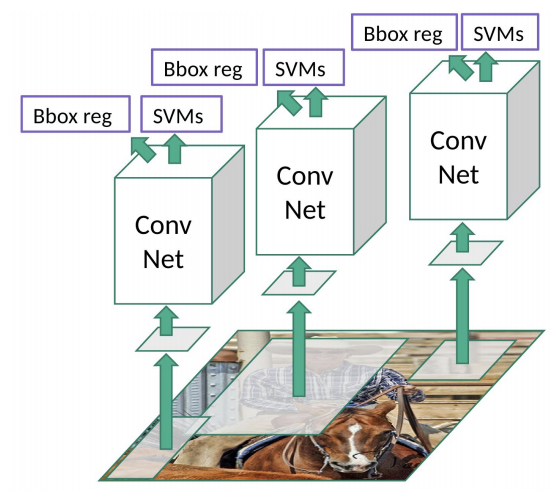
\includegraphics[width=8cm]{Bilder/rcnn.png} 
		\caption[R-CNN Architektur]{R-CNN Architektur \cite{RohithGandhi.20180709}}
		\label{rcnn}
	\end{center}
\end{figure}

Bei dem klassischen \textit{R-CNN} Detektor werden durch den \textit{Selective Search} Algorithmus 2000 solcher \textit{RoIs} vorgeschlagen. Zur Merkmalsextraktion wird für jede \textit{RoI} anschließend ein CNN eingesetzt. Der resultierende \textit{Feature Vektor} wird zur Klassifikation eines Objektes einer \textit{Support Vector Machine} unterzogen. Um zusätzlich die Bounding Boxen akkurat zu bestimmen, wird der \textit{Feature Vektor} zudem einem Bounding Box Regressor unterzogen (siehe Abbildung \ref{rcnn}) \cite{RohithGandhi.20180709}. 

Da der sogenannte \textit{Region Proposal} Schritt durch den \textit{Selective Search} Algorithmus allerdings viel Zeit in Anspruch nimmt, entstand eine Weiterentwicklung des \textit{R-CNN } Netzes, das \textit{Fast R-CNN} Netz. Dieses tauscht den Schritt des \textit{Selective Search} Algorithmus mit dem Einsatz des CNNs. Außerdem wird das klassische CNN leicht angepasst. Bei \textit{Fast R-CNN} wird ein Bild zunächst einem CNN unterworfen. Bevor eine \textit{Feature Map} durch \textit{Fully-Connected Layer} zu einem einzigen \textit{Feature Vektor} vereinfacht wird, werden aus der \textit{Feature Map} die verschiedenen \textit{RoIs} extrahiert. Dies geschieht wiederrum mit dem \textit{Selective Search} Algorithmus, mit dem Unterschied, dass dieser nun nur auf der \textit{Feature Map} operiert und nicht auf dem gesamten Bild. Durch \textit{RoI Pooling Layer} werden die einzelnen entstandenen Regionen in eine feste Größe transformiert und einzeln einer Klassifikation durch \textit{Fully-Connected Layer} und einer Softmax-Funktion unterworfen. Die Komponente mit dem \textit{Bounding Box Regressor} bleibt gleich. Durch den Tausch des CNNs mit dem \textit{Selective Search} Algorithmus werden die mathematischen Faltungsoperationen nur einmal statt 2000 Mal pro Bild ausgeführt, was die Performanz des Detektors gegenüber eines klassischen \textit{R-CNNs} enorm steigert \cite{RohithGandhi.20180709}.

\begin{figure}[ht]
	\begin{center}
		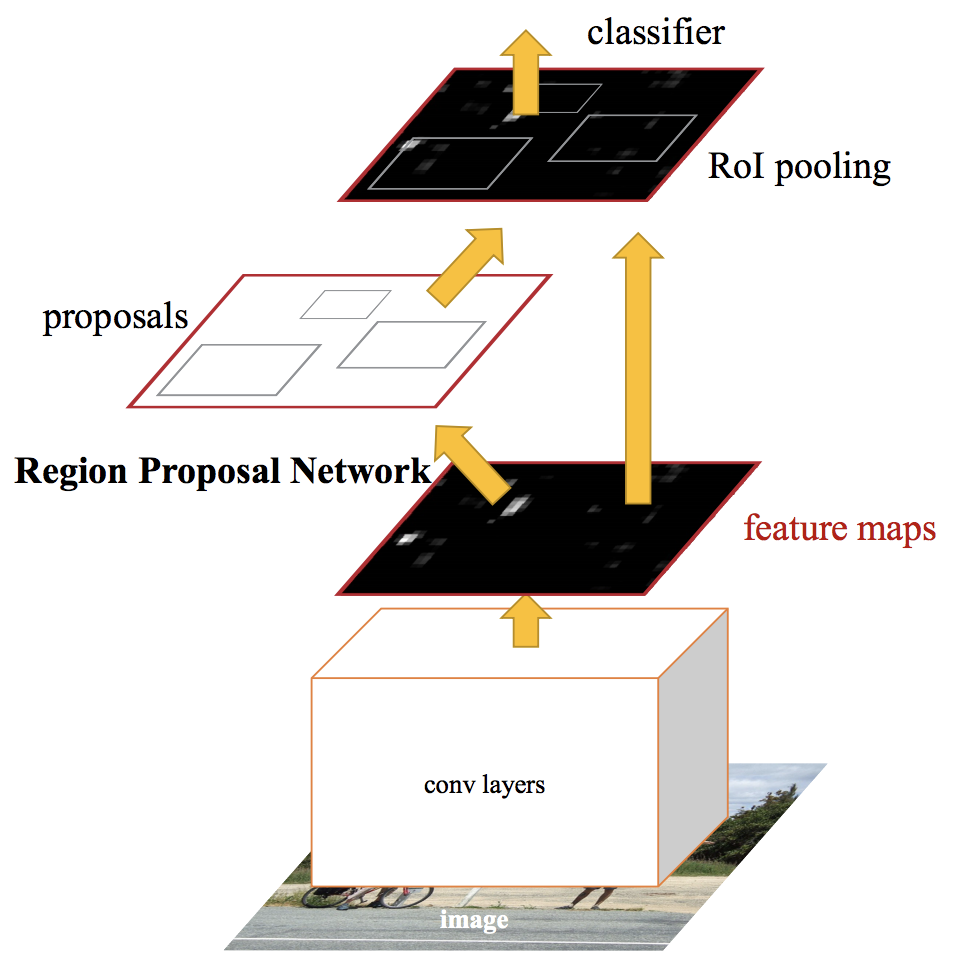
\includegraphics[width=8cm]{Bilder/fasterrcnn.png} 
		\caption[Faster R-CNN Architektur]{Faster R-CNN Architektur \cite{RohithGandhi.20180709}}
		\label{fasterrcnn}
	\end{center}
\end{figure}

Die letzte Optimierung der R-CNN Familie entstand durch das \textit{Faster R-CNN} Netz. Dieses ersetzt den statischen \textit{Selective Search} Algorithmus des \textit{Fast R-CNN} Detektors durch ein eigenes lernfähiges, sogenanntes \textit{Region Proposal Network} (RPN)  (siehe Abbildung \ref{fasterrcnn}) \cite{RohithGandhi.20180709}.

Neben dem Einsatz von RCNN Detektoren zur \textit{Objektdetektion} existiert ebenso ein Ansatz zur \textit{instanzbasierten Segmentierung}, das \textit{Mask R-CNN} Netz. Es nimmt zwei wichtige Anpassungen an der Architektur des \textit{Faster R-CNN} Netzes vor. Da bei Segmentierungsproblemen eine genauer Abgrenzung von Objekt und Hintergrund notwendig ist, wird das \textit{RoI Pooling Layer} durch ein \textit{RoI Align Layer} ausgetauscht. Hierbei wird das Rundungsproblem beim Pooling behoben. Angenommen eine \textit{RoI} von 16x16 Pixeln wird mit einem MEAN-Pooling Layer der Schrittweite Drei verarbeitet, so ergibt sich pro Pooling Schritt ein Einzugebegiet von 5.33 Pixeln. Dieses wurde abgerundet auf 5 Pixel. Bei \textit{RoI Align Layern} wird durch bilineare Interpolation der Wert des 5.33ten Pixels ermittelt und in das Pooling mit einbezogen. Dies ermöglicht eine genauere Segmentierung an den Grenzen eines Objektes \cite{UmerFarooq.20180215}.

Außerdem wird parallel zum RPN ein sogenanntes \textit{Fully Convolutional Network} (FCN) eingesetzt, einem Netz, dass rein aus \textit{Convolutional Layern} besteht. Es dient, um für jede existierende Klasse eine pixelbasierte binäre Maske auszugeben, die für jeden Pixel die Zugehörigkeit zu einer Klasse bestimmt. Basierend auf dieser Maske werden die detektierten Objekte anschließend farblich hervorgehoben \cite{DhruvParthasarathy.20170422}.